%%%%%%%%%%%%%%%%%%%%%%%%%%%%%%%%%%%%%%%%%%%%%%%%%%%%%%%%%%%%%%%%%%%%%%%%%%%%%%%%%%%%%%%%%%%%%%%%%%%%%%%
%%%%%%%%%%%%%% Template de Artigo Adaptado para Trabalho de Conclusão de Curso - SI Contagem - PUCMINAS %%%%%%%%%%%%%%%%%%%%%%%%
%% codificação UTF-8 - Abntex - Latex -  							     %%
%% Autor da primeira versão:    Fábio Leandro Rodrigues Cordeiro  (fabioleandro@pucminas.br)                            %% 
%% Co-autor da primeira versão: Prof. João Paulo Domingos Silva, Harison da Silva e Anderson Carvalho                   %%
%% Revisores normas NBR (Padrão PUC Minas) da primeira versão: Helenice Rego Cunha e Prof. Theldo Cruz                  %%
%% Versão: 1.1     18 de dezembro 2015                     	                                     %%
%%%%%%%%%%%%%%%%%%%%%%%%%%%%%%%%%%%%%%%%%%%%%%%%%%%%%%%%%%%%%%%%%%%%%%%%%%%%%%%%%%%%%%%%%%%%%%%%%%%%%%%


\documentclass[a4paper,12pt]{article}
\usepackage{times}
\usepackage{abakos}  %pacote com padrão da Abakos baseado no padrão da PUC
%%%%%%%%%%%%%%%%%%%%%%%%%%%
%Capa da revista
%%%%%%%%%%%%%%%%%%%%%%%%%%

%\setcounter{page}{80} %iniciar contador de pagina de valor especificado
\newcommand{\monog}{Modelo de artigo do Instituto de Ciências Exatas e de Informática}
%\newcommand{\monogES}{Article template Institute of Mathematical Sciences and Informatics}
\newcommand{\tipo}{Artigo}  % Especificar a seção tipo do trabalho: Artigo, Resumo, Tese, Dociê etc
%\newcommand{\origem}{Brasil}
%\newcommand{\editorial}{Belo Horizonte, p. 01-11, nov. 2024}  % p. xx-xx – páginas inicial-final do artigo
\newcommand{\editorial}{}  
\newcommand{\lcc}{\scriptsize{Licença Creative Commons Attribution-NonCommercial-NoDerivs 3.0 Unported}}

%%%%%%%%%%%%%%%%%INFORMAÇÕES SOBRE AUTOR PRINCIPAL %%%%%%%%%%%%%%%%%%%%%%%%%%%%%%%
\newcommand{\AutorA}{Nome completo do(a) aluno(a)}
\newcommand{\funcaoA}{}
\newcommand{\emailA}{\href{mailto:xxx@sga.pucminas.br}{xxx@sga.pucminas.br}}
\newcommand{\cursA}{Aluno(a) do Programa de Graduação em Sistemas de Informação}

\newcommand{\AutorB}{Nome completo do(a) orientador(a)}
\newcommand{\funcaoB}{}
\newcommand{\emailB}{\href{mailto:xxx@sga.pucminas.br}{xxx@pucminas.br}}
\newcommand{\cursB}{Professor(a) do Programa de Graduação em Sistemas de Informação}
% 
% Definir macros para o nome da Instituição, da Faculdade, etc.
\newcommand{\univ}{Pontifícia Universidade Católica de Minas Gerais}

\newcommand{\keyword}[1]{\textsf{#1}}

%Para as URLS não ultrapassarem a margem
\usepackage{url}
\makeatletter
\g@addto@macro{\UrlBreaks}{\UrlOrds}
\makeatother

\usepackage{adjustbox} % reduzir tamanho figuras

\usetikzlibrary{arrows,shapes,positioning,shadows,trees}

\tikzset{
  basic/.style  = {draw, text width=3cm, drop shadow, font=\sffamily, rectangle},
  root/.style   = {basic, rounded corners=2pt, thin, align=center,
                   fill=blue!30},
  level 2/.style = {basic, rounded corners=6pt, thin,align=center, fill=green!30,
                   text width=8em},
  level 3/.style = {basic, thin, align=left, fill=pink!60, text width=6.5em}
}

\begin{document}
% %%%%%%%%%%%%%%%%%%%%%%%%%%%%%%%%%%
% %% Pagina de titulo
% %%%%%%%%%%%%%%%%%%%%%%%%%%%%%%%%%%

\begin{center}

\includegraphics[scale=0.2]{figuras/brasao.jpg} \\
PONTIFÍCIA UNIVERSIDADE CATÓLICA DE MINAS GERAIS \\
Instituto de Ciências Exatas e de Informática

% \vspace{1.0cm}

\end{center}

 \vspace{0cm} {
 \singlespacing \Large{\monog \symbolfootnote[1]{Artigo apresentado ao Instituto de Ciências Exatas e Informática da Pontifícia Universidade Católica de \linebreak Minas Gerais, campus Contagem, como pré-requisito parcial para obtenção do título de Bacharel em Sistemas de Informação.} \\ }
 % \normalsize{\monogES}
 }

\vspace{1.0cm}

\begin{flushright}
\singlespacing 
\normalsize{\AutorA \footnote{\funcaoA \cursA \,-- \emailA . }} \\
\normalsize{\AutorB \footnote{\funcaoB \cursB \,-- \emailB . }} \\
%\normalsize{\AutorC \footnote{\funcaoC \cursC \,-- \emailC . }} \\
%\normalsize{\AutorD \footnote{\funcaD \cursD \,-- \emailD . }} \\
\end{flushright}
\thispagestyle{empty}

\vspace{1.0cm}

\begin{abstract}
\noindent
O resumo é redigido em parágrafo único. Um bom resumo deve conter uma frase para cada um dos tópicos: contexto, problema, justificativa, objetivo, desenvolvimento, resultados e conclusão do documento. Convém usar o verbo de forma impessoal. Seguindo o formato de artigo de periódico, o resumo deverá conter de 100 a 250 palavras. Evite o uso de símbolos e contrações que não sejam de uso corrente, bem como o uso de fórmulas, equações e referências que não sejam absolutamente necessários. Quando seu emprego for imprescindível, defini-los na primeira vez que aparecerem. Abaixo do resumo apresente a expressão ``Palavras-chave'' e, após os dois pontos, os termos com as iniciais em letra minúscula e separadas com ponto e vírgula (exceto para nomes próprios e científicos) e finalizadas por ponto final. 
\\\textbf{\keyword{Palavras-chave:}} template; \LaTeX; Abakos; periódicos.
\end{abstract}

%%%%%%%%%%%%%%%%%%%%%%%%%%%%%%%%%%%%%%%%%%%%%%%%%%%%%%%%%
\selectlanguage{english}
\begin{abstract}
\noindent
The abstract is written in a single paragraph. A good abstract should include the motivation, objective, methodology, results, and conclusion of the document. It is advisable to use impersonal verbs. Following the journal article format, the abstract should contain between 100 and 250 words. Avoid using symbols and contractions that are not commonly used, as well as formulas, equations, and references that are not absolutely necessary. When their use is essential, define them the first time they appear. Below the abstract, present the term ``Keywords'' and, after the colon, list the terms with lowercase initials separated by semicolons (except for proper and scientific names) and ending with a period.
\\\textbf{\keyword{Keywords:}} template; \LaTeX; Abakos; periodics.
\end{abstract}

\selectlanguage{brazilian}
 \onehalfspace  % espaçamento 1.5 entre linhas
 \setlength{\parindent}{1.25cm}

%%%%%%%%%%%%%%%%%%%%%%%%%%%%%%%%%%%%%%%%%%%%%%%%%
%% INICIO DO TEXTO
%%%%%%%%%%%%%%%%%%%%%%%%%%%%%%%%%%%%%%%%%%%%%%%%%

%%%%%%%%%%%%%%%%%%%%%%%%%%%%%%%%%%%%%%%%%%%%%%%%%%%%%%%%%%%%%%%%%%%%%%%%%%%%%%%%%%%%%%%%%%%%%%%%%%%%%%%%%%%%%%%%%%%%%%%%%%%%%%%%
%%%%%%%%%%%%%% Template de Artigo Adaptado para Trabalho de Conclusão de Curso - SI Contagem - PUCMINAS                       %%
%% codificação UTF-8 - Abntex - Latex -  							                                                          %%
%% Autor da primeira versão:    Fábio Leandro Rodrigues Cordeiro                                                              %% 
%% Co-autores da primeira versão: Prof. João Paulo Domingos Silva, Harison da Silva e Anderson Carvalho		                  %%
%% Revisores normas NBR (Padrão PUC Minas) da primeira versão: Helenice Rego Cunha e Prof. Theldo Cruz                        %%
%% Versão: 1.1     18 de dezembro 2015                                                                                        %%
%%%%%%%%%%%%%%%%%%%%%%%%%%%%%%%%%%%%%%%%%%%%%%%%%%%%%%%%%%%%%%%%%%%%%%%%%%%%%%%%%%%%%%%%%%%%%%%%%%%%%%%%%%%%%%%%%%%%%%%%%%%%%%%%
\section{\esp Introdução (1 - 2 páginas)} 

A formatação deverá ter parágrafo recuado a 1,25 centímetros, tamanho 12, fonte Arial ou Times New Roman, espaçamento entre linhas de 1,5cm e texto justificado. Os títulos dos capítulos devem utilizar a formatação caixa alta, negrito, tamanho 12. As seções e subseções devem devem seguir às normas ABNT.

Nesse sentido, este template já possui a formatação correta com margens, espaçamentos e tipo de folha requisitada no TCC. Quanto ao limite de páginas exigido no trabalho, são no mínimo 11 (onze) páginas e no máximo 15 (quinze) páginas, incluindo referências, anexos e apêndices.


A introdução deve conter 1 - 2 páginas, sendo um parágrafo para cada um dos tópicos:
	Contexto. Descrever o tema/área em que o trabalho se insere. 
	Ex.: A ocorrência de problemas psicológicos entre os adolescentes tem levado os educadores a se preocuparem com a possibilidade de que o mal uso das novas tecnologias possa estar provocando danos aos mesmos. A preocupação é agravada diante da constatação de que a maior parte dos adolescentes tem livre acesso aos conteúdos disponíveis na web \cite{citelli2004,martins2012}.
	
 Problema. Qual pergunta o seu trabalho procura responder? 
	Ex.: A inclusão digital nem sempre é realizada por meio das escolas, portanto ela pode ocorrer de uma forma não estruturada e sem o acompanhamento necessário. Mas mesmo quando a introdução às tecnologias, principalmente a informática, é realizada nas escolas, pode ocorrer o uso das mesmas pelos adolescentes sem o devido controle, fora das escolas. Como então a informática tem influenciado no processo de formação dos adolescentes?
	
 Justificativa. Por que essa pergunta é importante? Quais os benefícios você trará ao resolver este problema?
	Ex.: Ao determinar-se a influência da informática no processo de formação dos adolescentes, é possível elaborar estratégias de ensino que aproveitem as habilidades adquiridas pelos adolescentes para uma utilização correta e efetiva das tecnologias. Também pode-se identificar as dificuldades encontradas pelos adolescentes no uso da tecnologia e promover o aprendizado nas escolas, visando mitigar tais dificuldades.
	
 Objetivo. O que você fará neste trabalho? Como vai resolver o problema?
	Ex: O objetivo deste trabalho é realizar um estudo de caso da inclusão digital de adolescentes por meio de questionários para identificação da influência da informática no processo de formação destes adolescentes.
	
 Objetivos específicos. São detalhamentos do objetivo geral, que descrevem metas intermediárias a serem cumpridas para que o mesmo seja atingido.
	Ex.: São objetivos específicos deste trabalho: identificar escolas públicas de ensino médio na região metropolitana de Belo Horizonte, que ofereçam disciplinas introdutórias de informática na grade curricular; caracterizar o perfil socioeconômico dos estudantes das escolas identificadas...
	
 Estrutura do Trabalho. Descrever cada seção do seu trabalho.	
	Ex.: Este texto está estruturado em 5 seções. A seção 2 apresenta o referencial teórico… A seção 3 descreve os trabalhos relacionados. Na seção 4… Por último, ...


\section{\esp Referencial Teórico (2 - 3 páginas)}

Todo título de seção ou subseção deverá ser seguido de texto.  Para criar uma seção use \verb|\section{}|, e para as subseções use \verb|\subsection{}| e \verb|\subsubsection{}|. A ABNT permite até cinco níveis de subseções, no entanto, evite mais de dois níveis para melhor organização e fluidez do texto.


O Referencial Teórico deve se sustentar, preferencialmente, em publicações dos últimos 5 anos. O Referencial Teórico é organizado no formato de uma pirâmide. No topo, o tópico mais abrangente. Na base, o tópico mais específico. Ou seja, escreve-se menos sobre o tópico mais abrangente e mais sobre o tópico específico. Ex: Nesta seção são descritos os principais conceitos, classificações e técnicas relacionados a inclusão digital. 

\subsection{\esp Tópico mais abrangente (Ex.: Inclusão digital)} 
\label{subsec:1}
Por exemplo, para descrever o que é computação paralela, deve-se apresentar, pelo menos, três referências diferentes e escrever um parágrafo, com as suas próprias palavras, que resuma o que foi entendido das referências. Deve-se produzir um texto contínuo, de forma que as referências estejam concatenadas entre si.

As citações das referências podem ser diretas ou indiretas. As referências deverão ser adicionadas no arquivo \textit{bibliografia.bib}. Cada referência deverá ser adicionada conforme o padrão de normalização da PUC, 
o qual poderá ser consultado na página da biblioteca da \citeonline{manualpuc2023}. Todas as publicações citadas no texto deverão ter correspondente nas referências, 
e as indicações de autoria da citação e do ano deverão ser idênticas aos dados expostos. 

Para adequar-se à nova norma ABNT NBR 10520:2023, que não utiliza mais citações em caixa-alta, não exclua o arquivo \textit{abntex2-alf.bst} do seu projeto no Overleaf. É importante ressaltar que algumas entradas ainda podem apresentar inconformidades, como ao usar o comando \verb|\cite{}| para referências que possuem o campo \verb|@organization| preenchido, mas não têm o campo \verb|@author| ou o campo \verb|@editor| preenchido. A comunidade \texttt{abntex} está trabalhando em uma solução definitiva para esses casos.

\subsection{\esp Tópico intermediário (Ex.: Inclusão informacional) }
O mesmo procedimento descrito na Seção \ref{subsec:1} deve ser aplicado a cada parágrafo do capítulo do referencial teórico.

\subsection{\esp Tópico específico (Ex.: Inclusão social) }
O mesmo procedimento descrito na Seção \ref{subsec:1} deve ser aplicado a cada parágrafo do capítulo do referencial teórico.




\subsection{\esp Elementos flutuantes}

São elementos inseridos no texto como imagens, tabelas, algoritmos, etc.
De acordo com as normas ABNT, há a necessidade de se observar que todos os elementos flutuantes inseridos devem ter a formatação básica:

\begin{enumerate} [label={\alph*})]
 \item título centralizado localizado na parte superior; 
 \item fonte em tamanho 10 na parte inferior;
 \item se o elemento for de autoria própria, siga o exemplo do Quadro \ref{qua:quadro1}; caso contrário, faça a citação da referência conforme o exemplo da Figura \ref{fig:figura1}. Para elementos criados a partir de outros autores, usar a expressão  ``Adaptado de ...'' 
 \item devem ser inseridos o mais próximos do texto que os referenciam.
\end{enumerate}


\subsubsection{\esp Inserções de ilustrações}

As ilustrações devem ser inseridas seguindo o exemplo da Figura \ref{fig:figura1}. Nos casos de telas de software, estas também devem ser inseridas como figuras, e referenciadas no texto. Além disso, é necessário que seja citada no texto a empresa desenvolvedora, quando aplicável. 

% Figura
\begin{figure}[ht]
	\centering	
	\caption{Uma Grade Computacional como fonte transparente}
	\vspace{-0.4cm}
	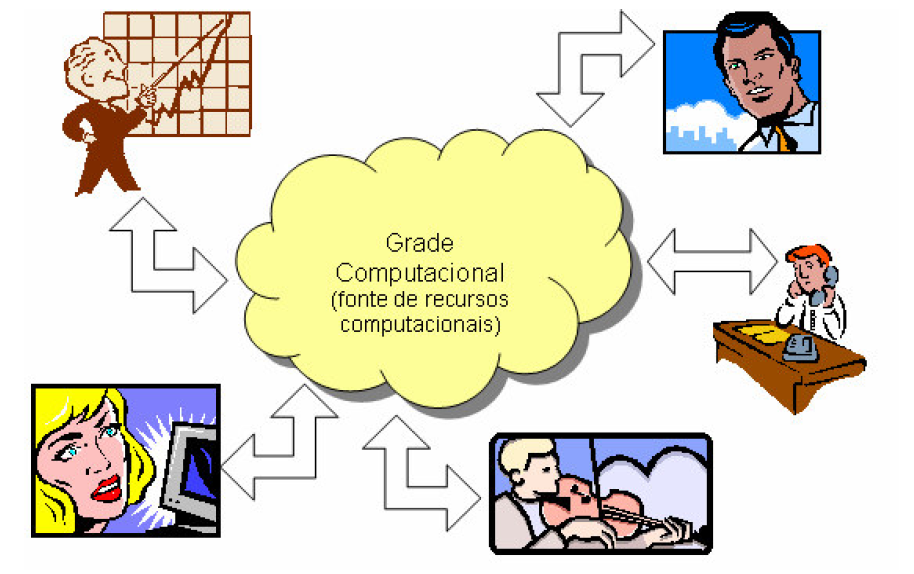
\includegraphics[width=0.7\textwidth]{figuras/grade-comp.png}
	% Caption centralizada
% 	\captionsetup{justification=centering}
	% Caption e fonte 
	 \vspace{-0.2cm}
	\\\textbf{\footnotesize Fonte: \citeonline{cap-livro2005} }
	\label{fig:figura1}
\end{figure}
\vspace{-0.5cm}

   \newpage

 \subsubsection{\esp Tabelas}

As tabelas devem ser abertas nas laterais, com espaços verticais separando
as colunas e sem espaços horizontais, exceto na
separação do cabeçalho. Um exemplo é a Tabela \ref{tab:tabela1}: 

% Tabela
\begin{table}[htb]
	\centering
	\caption{Exemplo de uma tabela}
	\vspace{-0.3cm} % espaço entre titulo e tabela
	\label{tab:tabela1}
	% Conteúdo da tabela
	\begin{tabular}{l|c|c}
  \hline
    \textbf{Imagem}	& \textbf{transferência} & \textbf{tempo} \\
    \hline
     estação 1	& 7,72 MB/s &  1:22:18 \\
     estação 2	& 7,72 MB/s &  1:22:17 \\
     estação 3	& 7,59 MB/s & 1:24:25 \\
     estação 4  & 7,53 MB/s & 1:43:27 \\
     estação 5	& 6,14 MB/s  &  1:24:41 \\
     estação 6  &  7,50 MB/s & 1:23:53 \\
     estação 7  & 7,58 MB/s  &  1:24:02 \\
     estação 8  & 7,8 MB/s  &  1:29:06 \\
     estação 9  & 7,9 MB/s  &  1:30:05 \\
     estação 10 & 8,0 MB/s  &  1:32:03 \\
     \hline
 \end{tabular}
 	\vspace{.1cm}  %espaço entre tabela e fonte
	\small
	% Fonte
	{\footnotesize\\ \textbf{Fonte: \citeonline{monografia2010}}}
\end{table}

\subsubsection{\esp Quadros}

Os quadros diferem das tabelas por apresentarem dados textuais.
Esses dados podem ser esquemáticos, comparativos ou descritivos.
  	
   	\begin{quadro}[H]
   		\centering
   		\caption{Bandas/Artistas de Rock e outros}
   	\label{qua:quadro1}
   		% Conteúdo do quadro
	\begin{tabular}{|c|c|c|c|} \hline
	\multicolumn{4}{|c|}{\textbf{Bandas ou Artistas de Rock e outros}} 	  \\ 
		\hline \textbf{	Progressivo} & Pink Floyd & Jethro Tull	& Yesterday \\ 
		 \hline \textbf{ Metal}  & Metallica & Iron Maidam & Black Sabath \\ 
		\hline \textbf{	Arena Rock} & Led Zeppelin & The Rolling Stones & Beatles \\ 
		\hline \textbf{ Punk} & Ramones & Black Flag & NOFX	\\ 
		\hline \textbf{	Nacional} & Ira & Engenheiros & Vinil	\\ 
		\hline \textbf{	S.J.E.} & Apolo XI & Invasão 7 & Por do Sol \\ 
		\hline \textbf{	Grunge} & Nirvana & Pear Jam & Alice in Chains	\\ 
		\hline \textbf{	Rock Folk} & Bod Dylan & The Byrds &  The Mamas \& the Papas \\
		\hline \textbf{	Blues} & B.B. King & Albert Colins & Mady Wathers \\ 
		\hline \textbf{	New Wave} & The Police & The Pretenders, &  Duran Duran\\ 
 		\hline \textbf{	Rock Folk} & Bod Dylan & The Byrds &  The Mamas \& the Papas \\
 		\hline \textbf{	Rock alternativo} & R.E.M.& Hüsker Dü & Big Black\\ 
		\hline
	\end{tabular}
	\vspace{.1cm}  %espaço entre quadro e fonte
	\small
	% Fonte
	{\footnotesize\\ \textbf{Fonte: Elaborado pelo autor}}
   \end{quadro}

   
\subsubsection{\esp Inserção de algoritmos}

Para inserir um algoritmo, utilizar o exemplo do Algoritmo  \ref{alg:rnagenerica}.
Todos os algoritmos devem ser inseridos assim como é feito para figuras, tabelas, ou seja, devem ser indicados por nome e fonte.


\begin{center}	
    \textbf{Algoritmo 1 -  CAC RD Neural}
	\vspace{-0.3cm}
\begin{minipage}[ht]{13cm}
\begin{algorithm}[H]
  \footnotesize
  \caption{CAC-RD Neural}
  \label{alg:rnagenerica}
  \begin{algorithmic}[1]
      \STATE \textbf{Entrada:} Requisição da chamada
    \STATE \textbf{Saída:} Aceitação ou bloqueio da solicitação
    
    \STATE Preenche o vetor de $attributes.size+1$ atributos com os valores dos atributos, sendo a primeira posição do vetor preenchida com o valor 1
		\STATE $hidden\_layer\_size =  attributes.size*2+1;$

    \FOR{$i$ = 1 to $attributes.size+1$}
    	\STATE \textbf{normalizar}($Entrada_i$)
    \ENDFOR

		\STATE $double [] net = new double [hidden\_layer\_size];$
    \STATE $net = hidden\_layer\_weights * attributes;$
   	\FOR{$i$ = 0 to hidden\_layer\_size}
			\STATE $net [i] = 1.0 / (1.0 + exp((-1.0)*net[i]));$
		\ENDFOR

		\STATE $double [] ipVector = new double [hidden\_layer\_size+1];$
    \STATE $ipVector [0] = 1.0;$
   	\FOR{$i$ = 1 to $hidden\_layer\_size+1$}
			\STATE $ipVector [i] = net [i-1];$
		\ENDFOR
		
		\STATE $output = output\_layer\_weights *  ipVector;$
    \STATE output = \textbf{desnormalizar}(Saída)
    \STATE \textbf{net\_update} (requisition);
    
    \STATE \textbf{Retorna} output; FIM
  \end{algorithmic}
\end{algorithm}
% \vspace{-0.3cm} % espaço entre algoritmo e fonte

\small \centering \textbf{\footnotesize Fonte: \citeonline{mestrado2010}.}
\end{minipage}
\end{center}
% \end{figure}
   
\section{\esp Trabalhos Relacionados (1 página)}

A seção de Trabalhos Relacionados deve apresentar um pequeno resumo (um parágrafo) de cada artigo, monografia ou demais trabalhos que tenham feito algo parecido com o seu trabalho. Em seguida, devem ser destacadas as diferenças e semelhanças entre o seu trabalho e o relacionado. Devem ser apresentados no mínimo 3 trabalhos relacionados. Os trabalhos relacionados não devem ter sido usados como referências no capítulo anterior.

Lembre-se de usar corretamente a formatação para citações. As citações podem ser classificadas como livres, diretas ou citação de citação, esta última não abordada neste documento.


\subsection{\esp Citação livre ou indireta}

Quando se reproduzir ideias, sem transcrever as palavras do autor, a indicação da página é opcional. Exemplos desse tipo de citação:
\begin{enumerate} 
 \item citação com um autor \cite{knuth1968}. 
 \item citação de artigos em revistas com dois autores \cite{prenner2022}.\footnote{Quando citar um artigo, inclua o DOI (Identificador de Objeto Digital) sempre que estiver disponível.}
  \item trabalho em congresso com três autores \cite{vasconcelos2016}.
 \item trabalhos com mais de três autores \cite{cap-livro2005}.
 \item citação de dois autores de uma vez em duas obras distintas \cite{gil2022,groupp2003}.
\end{enumerate}

\subsection{\esp Citação direta ou textual}

Transcrição literal de textos de outros autores. Nesse caso, deverão ser especificadas as páginas consultadas. 


\subsubsection{\esp Textual curtas}

Quando curtas (até 3 linhas) serão inseridas na sequência normal do texto, entre aspas duplas com as mesma formatação.

\subsubsection{\esp Textual longas}

Citações longas (mais de 3 linhas) deverão constituir um parágrafo independente, recuado a 4 cm da margem esquerda, 
com letra tamanho 10 e digitado em espaço simples, sem aspas.
\begin{citacaodireta}
Hegel chama trabalho à forma específica da satisfação das necessidades, que
distingue da natureza o espírito existente. Assim como a linguagem infringe
a imposição da intuição e ordena o caos das múltiplas sensações em coisas
identificáveis, assim o trabalho infringe a imposição do \hspace{0.1cm}desejo \hspace{0.1cm}imediato \hspace{0.1cm}e
suspende, por assim dizer, o processo de satisfação das necessidades.
\cite[25]{habermas1997}.
\end{citacaodireta}


% Artigo \cite{whatershed:01}

\subsubsection{\esp Textual de outros idiomas (tradução)}

Quando a citação estiver em outro idioma e for traduzida, indique após a chamada da citação a expressão tradução nossa ou tradução própria, entre parênteses. Obs: Em nota de rodapé informe, se desejar, a citação direta no idioma consultado.

\begin{citacaodireta} 
Um cluster é um computador paralelo construído de componentes e processos de software (tal como sistema de software). 
Um cluster é formado de nós, cada um contendo um ou mais processadores, memória que é compartilhada por todos os processadores do nodo 
(somente eles), e dispositivos periféricos adicionais (tais como discos), conectados pela rede e que permitem tráfego de dados entre os nós...
\cite[p. 10, tradução nossa]{groupp2003}\footnote {... a cluster is a parallel computer that is constructed of commodity  components and runs 
(as its system software) commodity software. A cluster is made of nodes, each 
containing one or more processors, memory that is  shared 
by all of the processors in (and only on) the node, and additional peripheral devices (such as disks), connected by network that allows data to move between the nodes.}.
\end{citacaodireta}
 
\subsection{\esp Exemplos de citações} 

Seguem alguns exemplos de citações mais utilizadas e/ou que geram algumas dúvidas. É válido observar que não serão citadas aqui
todas as possibilidades de citações. Sendo assim é de extrema relevância que se consulte o documento no site da Biblioteca (\citeonline{manualpuc2023}) para maiores esclarecimentos acerca de citações.

\subsubsection{\esp Citação de monografia, dissertação e tese}

Um exemplo de citação de monografia de curso de graduação ou especialização pode ser visto em \citeonline{monografia2010}.
Já para dissertação de mestrado veja \citeonline{mestrado2010}. E para o doutorado a citação é feita da seguinte forma: \citeonline{tese2012}. 



\subsubsection{\esp Livros e partes de livros}

Exemplo de capítulo de livro fica conforme esse exemplo: \cite{cap-livro2005}.

Para livros citados no corpo do texto e com duas citações juntas, ver os exemplos: \citeonline{knuth1968,groupp2003}.

\newpage

\section{\esp Metodologia (1 - 2 páginas)}
A Metodologia descreve o tipo e as etapas da pesquisa, estabelecendo um plano detalhado para a coleta e análise de dados. Além disso, uma metodologia bem definida permite a replicação do estudo, contribui para a transparência dos procedimentos e facilita a interpretação e aplicação dos achados.

    \subsection{\esp Classficação da pesquisa}
As pesquisas podem ser classificadas de diversas formas, como pode ser visualizado na Figura \ref{fig:metodologia}. Para mais informações sobre tais classificações, consulte materiais como \citeonline{gil2022,wazlawick2021}.

\begin{figure}[H]
    \centering
    \caption{Classificação das pesquisas científicas \citeonline{gil2022}}
    \begin{adjustbox}{valign=c}
		\resizebox{0.85\textwidth}{!}{ % para ajustar o tamanho da figura
    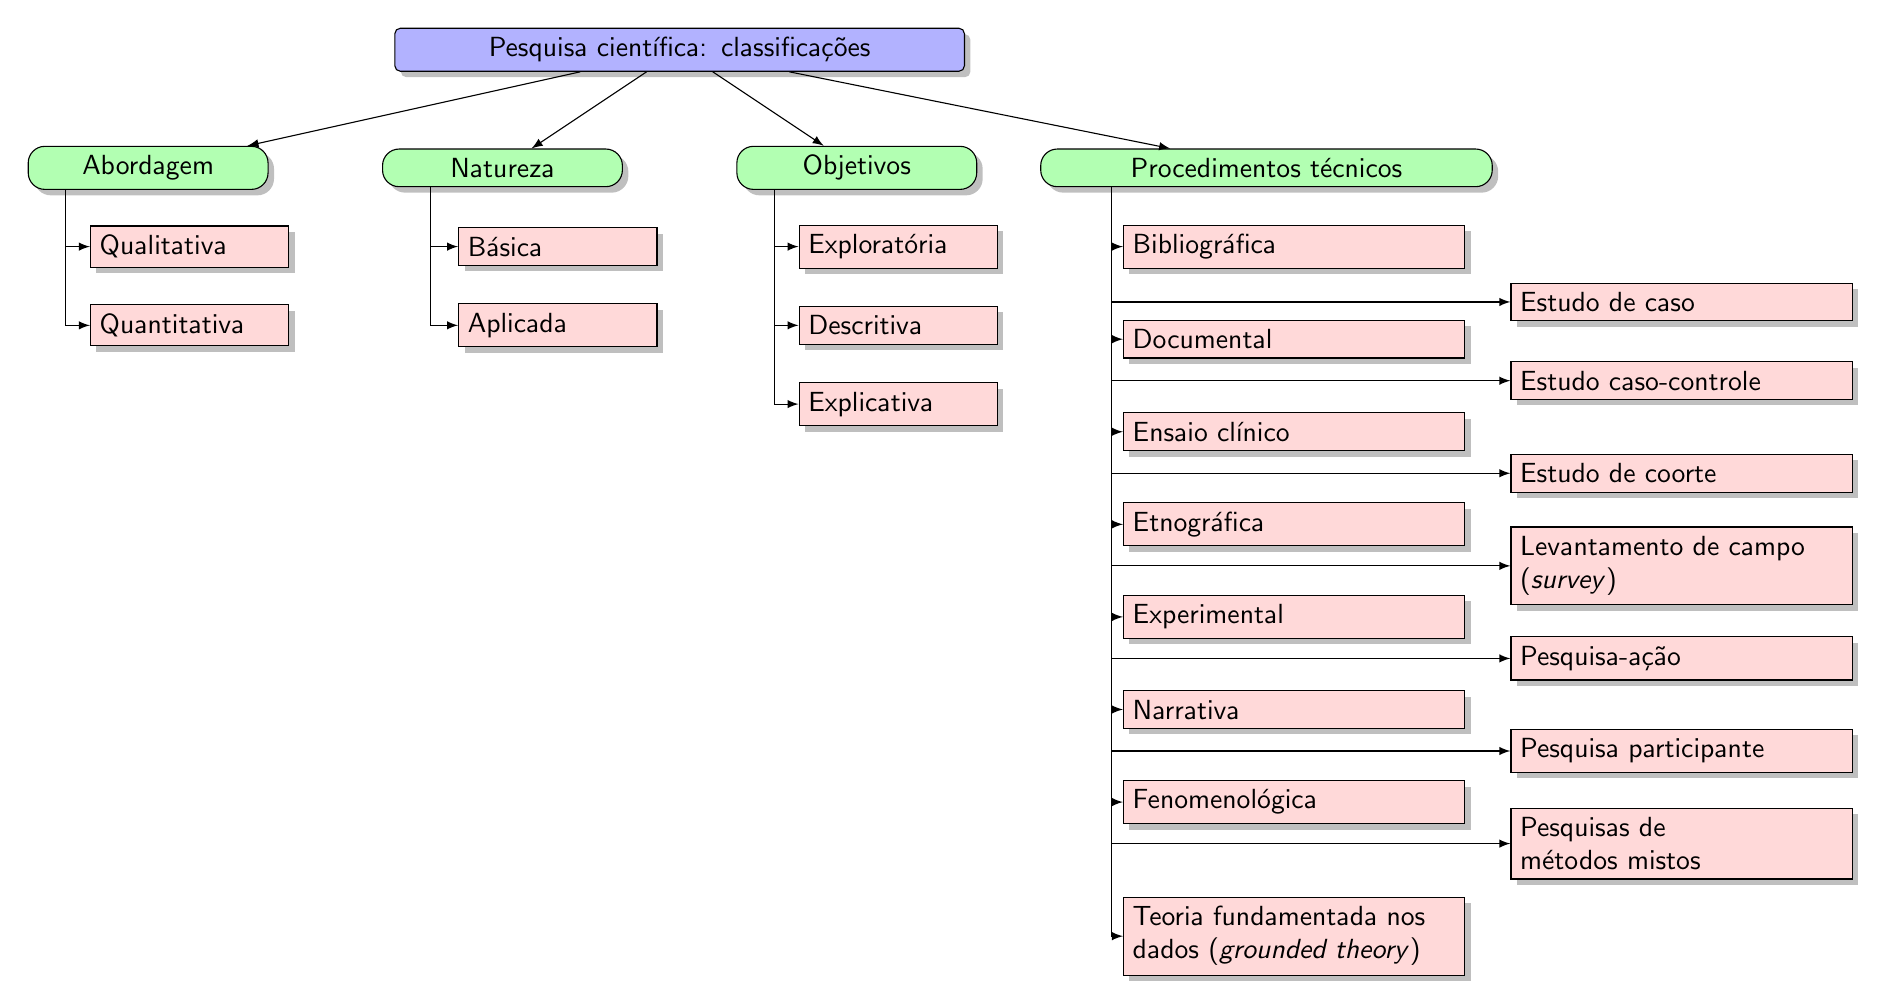
\begin{tikzpicture}[
  level 1/.style={sibling distance=45mm},
  edge from parent/.style={->,draw},
  >=latex]

% root of the the initial tree, level 1
\node[root,text width=7cm] {Pesquisa científica: classificações}
% The first level, as children of the initial tree
  child {node[level 2] (c1) {Abordagem}}
  child {node[level 2] (c2) {Natureza}}
  child {node[level 2] (c3) {Objetivos}}
  child {node[level 2, xshift=20pt, text width=5.5cm] (c4) {Procedimentos técnicos}};
;

% The second level, relatively positioned nodes
\begin{scope}[every node/.style={level 3}]
\node [below of = c1, xshift=15pt] (c11) {Qualitativa};
\node [below of = c11] (c12) {Quantitativa};

\node [below of = c2, xshift=20pt] (c21) {Básica};
\node [below of = c21] (c22) {Aplicada};

\node [below of = c3, xshift=15pt] (c31) {Exploratória};
\node [below of = c31] (c32) {Descritiva};
\node [below of = c32] (c33) {Explicativa};
\node [below of = c4, xshift=10pt, text width=4.1cm] (c41) {Bibliográfica};
\node [below of = c41, yshift=-5pt, text width=4.1cm] (c42) {Documental};
\node [below of = c42, yshift=-5pt, text width=4.1cm] (c43) {Ensaio clínico};
\node [below of = c43, yshift=-5pt, text width=4.1cm] (c44) {Etnográfica};
\node [below of = c44, yshift=-5pt, text width=4.1cm] (c45) {Experimental};
\node [below of = c45, yshift=-5pt, text width=4.1cm] (c46) {Narrativa};
\node [below of = c46, yshift=-5pt, text width=4.1cm] (c47) {Fenomenológica};
\node [below of = c47, yshift=-20pt, text width=4.1cm] (c48) {Teoria fundamentada nos dados (\textit{grounded theory})};
\node [below of = c4, xshift=150pt, yshift=-20pt, text width=4.1cm] (c49) {Estudo de caso};
\node [below of = c49, yshift=0pt, text width=4.1cm] (c410) {Estudo caso-controle};
\node [below of = c410, yshift=-5pt, text width=4.1cm] (c411) {Estudo de coorte};
\node [below of = c411, yshift=-5pt, text width=4.1cm] (c412) {Levantamento de campo (\textit{survey})};
\node [below of = c412, yshift=-5pt, text width=4.1cm] (c413) {Pesquisa-ação};
\node [below of = c413, yshift=-5pt, text width=4.1cm] (c414) {Pesquisa participante};
\node [below of = c414, yshift=-5pt, text width=4.1cm] (c415) {Pesquisas de \linebreak métodos mistos};
\end{scope}



% lines from each level 1 node to every one of its "children"
\foreach \value in {1,2}
  \draw[->] (c1.195) |- (c1\value.west);

\foreach \value in {1,...,2}
  \draw[->] (c2.195) |- (c2\value.west);

\foreach \value in {1,...,3}
  \draw[->] (c3.195) |- (c3\value.west);

 \foreach \value in {1,...,15}
   \draw[->] (c4.195) +(-30pt,0) |- (c4\value.west);
\end{tikzpicture}}
\end{adjustbox}
	\vspace{.1cm}  %espaço entre figura e fonte
	\\\textbf{\footnotesize Fonte: Elaborada pelo autor}  
 \label{fig:metodologia}
\end{figure}

É importante esclarecer em quais tipos de pesquisa o seu estudo se enquadra.
Ex: Este trabalho apresenta uma pesquisa de natureza qualitativa, que, a partir de dados coletados por meio de entrevistas e questionários, os analisa, classifica e interpreta.

\subsection{\esp Etapas da pesquisa}

	Nesta subseção, deve-se descrever as etapas para a realização da pesquisa. Como foi identificada e selecionada a amostra? Como foi feita a elaboração e aplicação dos questionários da pesquisa? Cada etapa deve ser detalhada.

\newpage
Ex: Esta pesquisa é dividida nas seguintes etapas:

\begin{enumerate}
\item levantamento bibliográfico;
\item elaboração de questionários;
\item estruturação e definição das entrevistas;
\item aplicação dos questionários e entrevistas;
\item apresentação, interpretação e análise dos resultados obtidos.
\end{enumerate}

Na elaboração dos questionários, foram levantados os principais fatores que podem influenciar na formação dos adolescentes e as ferramentas possivelmente utilizadas. Para cada um desses fatores, foram elaboradas questões de múltipla escolha e abertas. O questionário foi respondido por 30 pessoas, sendo 10 pessoas de cada classe social (baixa, média e alta). A determinação de classe social foi feita utilizando-se o Critério Brasil de Classificação Social.


\section{\esp Resultados (3 - 5 páginas)}

Nos Resultados você deve apresentar os gráficos com os resultados obtidos e também analisá-los. Note que apresentar é apenas descrever o que pode ser visto no gráfico, enquanto que analisar significa explicar o porquê dos resultados apresentados (essa explicação deve ser sustentada por dados da pesquisa. Caso não seja, deve-se deixar claro que se trata se uma possibilidade não comprovada).


Ex: O Quadro \ref{qua:quadro2} apresenta a quantidade de adolescentes que utilizam computador nas escolas. Pode-se observar que todos os alunos da classe alta utilizam computadores na escola, comparado com apenas 30\% dos alunos da classe baixa. (apresentação)

\begin{quadro}[H]
   		\centering
   		\caption{Quantidade de adolescentes que utilizam computador nas escolas}
   	\label{qua:quadro2}
   		% Conteúdo do quadro
\begin{tabular}{|c|C{3cm}|C{3cm}|}
\hline
\multirow{2}{*}{\textbf{Classe}} & \multicolumn{2}{c|}{\textbf{Você utiliza computador na escola?}} \\ \cline{2-3} 
                                 & \textbf{Sim} & \textbf{Não} \\ \hline
Baixa                            & 3            & 7            \\ \hline
Média                            & 8            & 2            \\ \hline
Alta                             & 10           & 0            \\ \hline
\end{tabular}
	\vspace{.1cm}  %espaço entre quadro e fonte
	\small
	% Fonte
	{\footnotesize\\ \textbf{Fonte: Elaborado pelo autor}}
   \end{quadro}

Ex: Na classe média, 20\% dos alunos não utilizam computadores nas escolas. Este resultado se deve ao fato que estes dois adolescentes estudam em escolas públicas. Apesar disso, todos os alunos da classe baixa estudam em escola pública, mas 30\% delas possuem aulas de informática. (análise)


\section{\esp Conclusão (1 página)}


É o capítulo de encerramento do trabalho, que contém a discussão dos resultados obtidos na pesquisa. É onde se colocam as observações do autor.  A conclusão deve estar de acordo com os objetivos do trabalho. Ela não deve apresentar citações ou interpretações de outros autores.

Sendo assim, uma conclusão é composta de:
	Conclusão Geral. Síntese do que foi realizado. Os objetivos foram alcançados totalmente? Os resultados foram compatíveis com as expectativas?
	Ex: Este trabalho apresentou um estudo de caso da inclusão digital de adolescentes, realizado por meio da análise de questionários, que foram aplicados para identificação da influência da informática no processo de formação destes adolescentes. Os resultados mostram que os adolescentes de classe baixa com acesso a informática ainda são uma minoria.
	
 Discussão dos Resultados. Extrapolação dos resultados obtidos (e se...); destaque das limitações, vantagens e desvantagens da pesquisa, entre outras observações.
	Ex: Nesta pesquisa não foi analisado o impacto da informática na formação de crianças e jovens. Apesar disso, os resultados poderiam ser estendidos para estas diferentes faixas etárias.
	
 Contribuições da Pesquisa. Metas alcançadas, ou seja, os objetos importantes produzidos.
	Ex: A principal contribuição desta pesquisa foi identificar que adolescentes são excluídos do mundo digital principalmente pela falta de aulas de informática nas escolas públicas, independente da classe econômica.
	
 Trabalhos Futuros. Possíveis evoluções da pesquisa, sugestões de pesquisas relacionadas etc.
	Ex: Como trabalhos futuros, pretende-se realizar um estudo de caso do impacto da informática na formação de crianças e jovens. Além disso, pretende-se fazer um estudo sobre a inclusão digital mais restrita aos adolescentes estudantes de escolas públicas.




%%%%%%%%%%%%%%%%%%%%%%%%%%%%%%%%%%%
%% FIM DO TEXTO
%%%%%%%%%%%%%%%%%%%%%%%%%%%%%%%%%%%

% \selectlanguage{brazil}
%%%%%%%%%%%%%%%%%%%%%%%%%%%%%%%%%%%
%% Inicio bibliografia
%%%%%%%%%%%%%%%%%%%%%%%%%%%%%%%%%%%

 \newpage
\singlespace{
\renewcommand\refname{REFERÊNCIAS}
\bibliography{bibliografia}
}

%Inclusão do arquivo abntex2-alf.bst como solução para adequação à ABNT NBR 10520:2023 quanto às citações, que não são mais em caixa-alta
\bibliographystyle{abntex2-alf.bst}

\end{document}
